\documentclass[12pt,a4paper]{report}
\usepackage[T1]{fontenc}
\usepackage[utf8]{inputenc}
\usepackage{charter}
\usepackage{ngerman}
\usepackage[left=2cm,right=2cm,top=2cm,bottom=2cm]{geometry}
\usepackage{graphicx}
\usepackage{amsmath}
\usepackage{tikz}
\usepackage{pgfplots}

\renewcommand\thesection{1.\arabic{section}} 

\begin{document}
	\setcounter{section}{12}
	\section{Grundgleichung für Wellenüberlagerungen}
	Wir haben \dq gesehen\dq, dass es Stellen im Raum gibt, an denen sich Wellen (bei der Aussendung identischer Wellen kit der Wellenlänge $\lambda$ von zwei Sendern) überlagern und hierbei auslöschen bzw. verstärken können. Betrachten wir dazu folgende Skizze:\\\\
	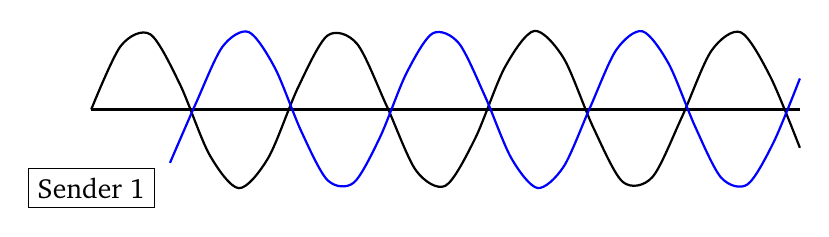
\begin{tikzpicture}
		\draw[thick] (0,0) -- (9,0);
		\draw[thick,black,smooth] (0,0) plot[domain=0:9] ({\x}, {sin(2.5*\x r)});
		\draw[thick,blue,smooth] (0,0) plot[domain=1:9] ({\x}, {cos(2.5*(\x+3.1) r)});
		\node[draw] at (0,-1) {Sender 1};
	\end{tikzpicture}\\\\
	\includegraphics[width=\textwidth]{JPEG-Bild-443E-8313-20-0.JPEG}
	Eine Auslöschung (\dq Destruktive Interferenz\dq) erhalten wir, wenn wir die beiden Sender um eine halbe Wellenlänge (+ Vielfaches einer Wellenlänge) von uns entfernt stehen:
	\begin{align*}
		\bigtriangleup =n \cdot \lambda + \frac{\lambda}{2} &= \lambda \cdot (n+\frac{1}{2})
	\end{align*} \\
	Gangunterschied $\bigtriangleup$: \dq Weglängendifferenz\dq \\
	\includegraphics[width=\textwidth]{JPEG-Bild-4CCB-9E90-7A-0.JPEG}
	\newpage
	\paragraph{konstruktive Interferenz}:
	\mbox{} \\
	Um eine konstruktive Interferenz zu erzeugen, muss der zweite Sender um n volle Wellenlänge verschoben sein (auch 0 möglich).
	\\\\
	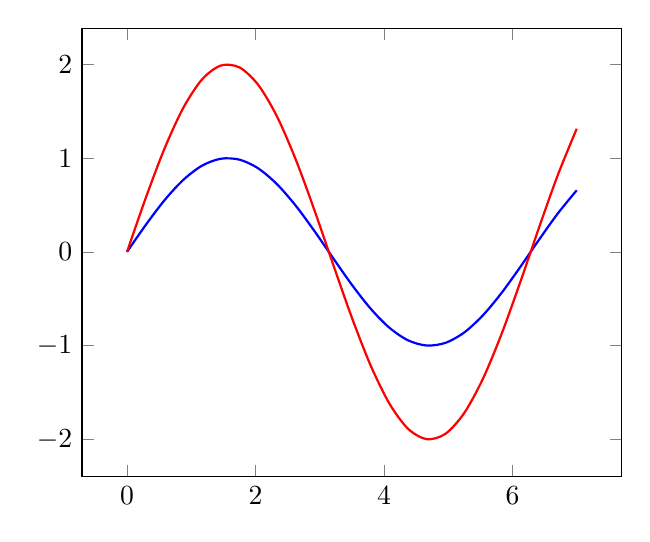
\begin{tikzpicture}
		\begin{axis}[domain=0:7]
			\addplot[smooth,thick,blue]{sin(deg(x))};
			\addplot[smooth,thick,red]{2*sin(deg(x))};
		\end{axis}
	\end{tikzpicture}
	\\\\
	Gangunterschied bei konstruktiver Interferenz: \\
	\begin{align*}
		\bigtriangleup &= n \cdot \lambda \\
		n &= \{0;1;2;...\}
	\end{align*}
	
	\section{Brechung bei Mikrowellen}
	\paragraph{Versuchsaufbau}: \mbox{} \\\\
	\begin{tikzpicture}
		\draw (2,1) -- (2,2);
		\draw (2,1) -- (3,1.25);
		\draw (2,2) -- (3,1.75);
		\draw (3,1.25) -- (3,1.75);
		\node[draw] at (2,3) {Mikrowellensender};
		\draw[->] (3,1.5) -- (5,0.25);
		\draw (4,-1) -- (6,1.5);
		\draw (6,1.5) -- (8,-1);
		\draw (4,-1) -- (8,-1);
		\node[draw] at (6,-1.5) {Prisma};
		\draw (5,0.25) -- (7,0.25);
		\draw[->] (7,0.25) -- (9,0);
		\draw (9,0.5) -- (9,-0.5);
		\draw (9,0.5) -- (10,1);
		\draw (9,-0.5) -- (10,-1);
		\draw (10,1) -- (10,-1);
		\node[draw] at (12.5,0) {Mikrowellensender};
		\node[draw] at (9,-3) {Signal wird gebrochen};
		\draw[->] (8.4,-2.7) -- (8.4,0);
	\end{tikzpicture} 
	\paragraph{Beobachtungen}: \mbox{} \\
	Setzen wir ein Plexiglas-prisma in den Raum zwischen Sender und Empfänger, wird das Signal deutlich schwächer.
	Verschiebe ich den Empfänger, so finde ich eine Stelle, bei der der Signalempfang wieder stärker ist.
\end{document}